\documentclass{beamer}
\usepackage{tbagrelbeamer}
\usepackage{beamerstyleceylan}

\newcommand{\tech}[1]{{\small \sc{#1}}}
\newcommand{\relief}[1]{{\color{structureTextColor} #1}}
\newcommand{\blue}[1]{{\color{regularblue} #1}}
\newcommand{\green}[1]{{\color{regulargreen} #1}}

\newcommand{\noeud}[1]{\blue{#1}}
\newcommand{\bit}[1]{{\small \bf{\tt{\green{#1}}}}}
\newcommand{\feuille}[2]{\bf{\tt{\large #2}}~|~\tt{\blue{#1}}}

\usetikzlibrary{arrows.meta}


\theoremstyle{theoreme}
\newtheorem{theoreme}{Théorème.~}

\title{Les données sont D\tss{1}}
\subtitle{\'Etude de méthodes de compression sans pertes}
\author{Thomas \sc{Bagrel}}
\institute{Lycée Henri \sc{Poincaré}, Nancy}
\date{\sc{tipe} session 2018}

\begin{document}

% \begin{frame}
%   \frametitle{\secname{}}
%   \framesubtitle{\subsecname{}}

% \end{frame}

\begin{frame}
  \titlepage{}
\end{frame}

\begin{frame}
  \frametitle{Aperçu}

  \tableofcontents % [pausesections]
\end{frame}

\section{Régularités et gains}

\subsection{Théorie}

\begin{frame}
  \frametitle{\secname{}}
  \framesubtitle{\subsecname{}}

  \relief{Compression des données sans pertes}
  \begin{itemize}
    \item \pause exploiter les régularités des données
    \item \pause données aléatoires : pas de gain
  \end{itemize}

  \pause
  \begin{theoreme}[Entropie de \sc{Shannon}]
  \[
    H(S) = -\sum_{i = 1}^n p_i \log_2(p_i)
  \]
  {\footnotesize $H(S)$ : nb. de bits moyen par symbole de la source }
  \end{theoreme}
  \begin{itemize}
    \item \pause une fois les données compressées (dérivées) une fois, plus aucune régularité
  \end{itemize}
\end{frame}

\subsection{\tech{zip} recursif}

\begin{frame}
  \frametitle{\secname{}}
  \framesubtitle{\subsecname{}}

  \vspace{-0.43cm}

  \begin{center}
    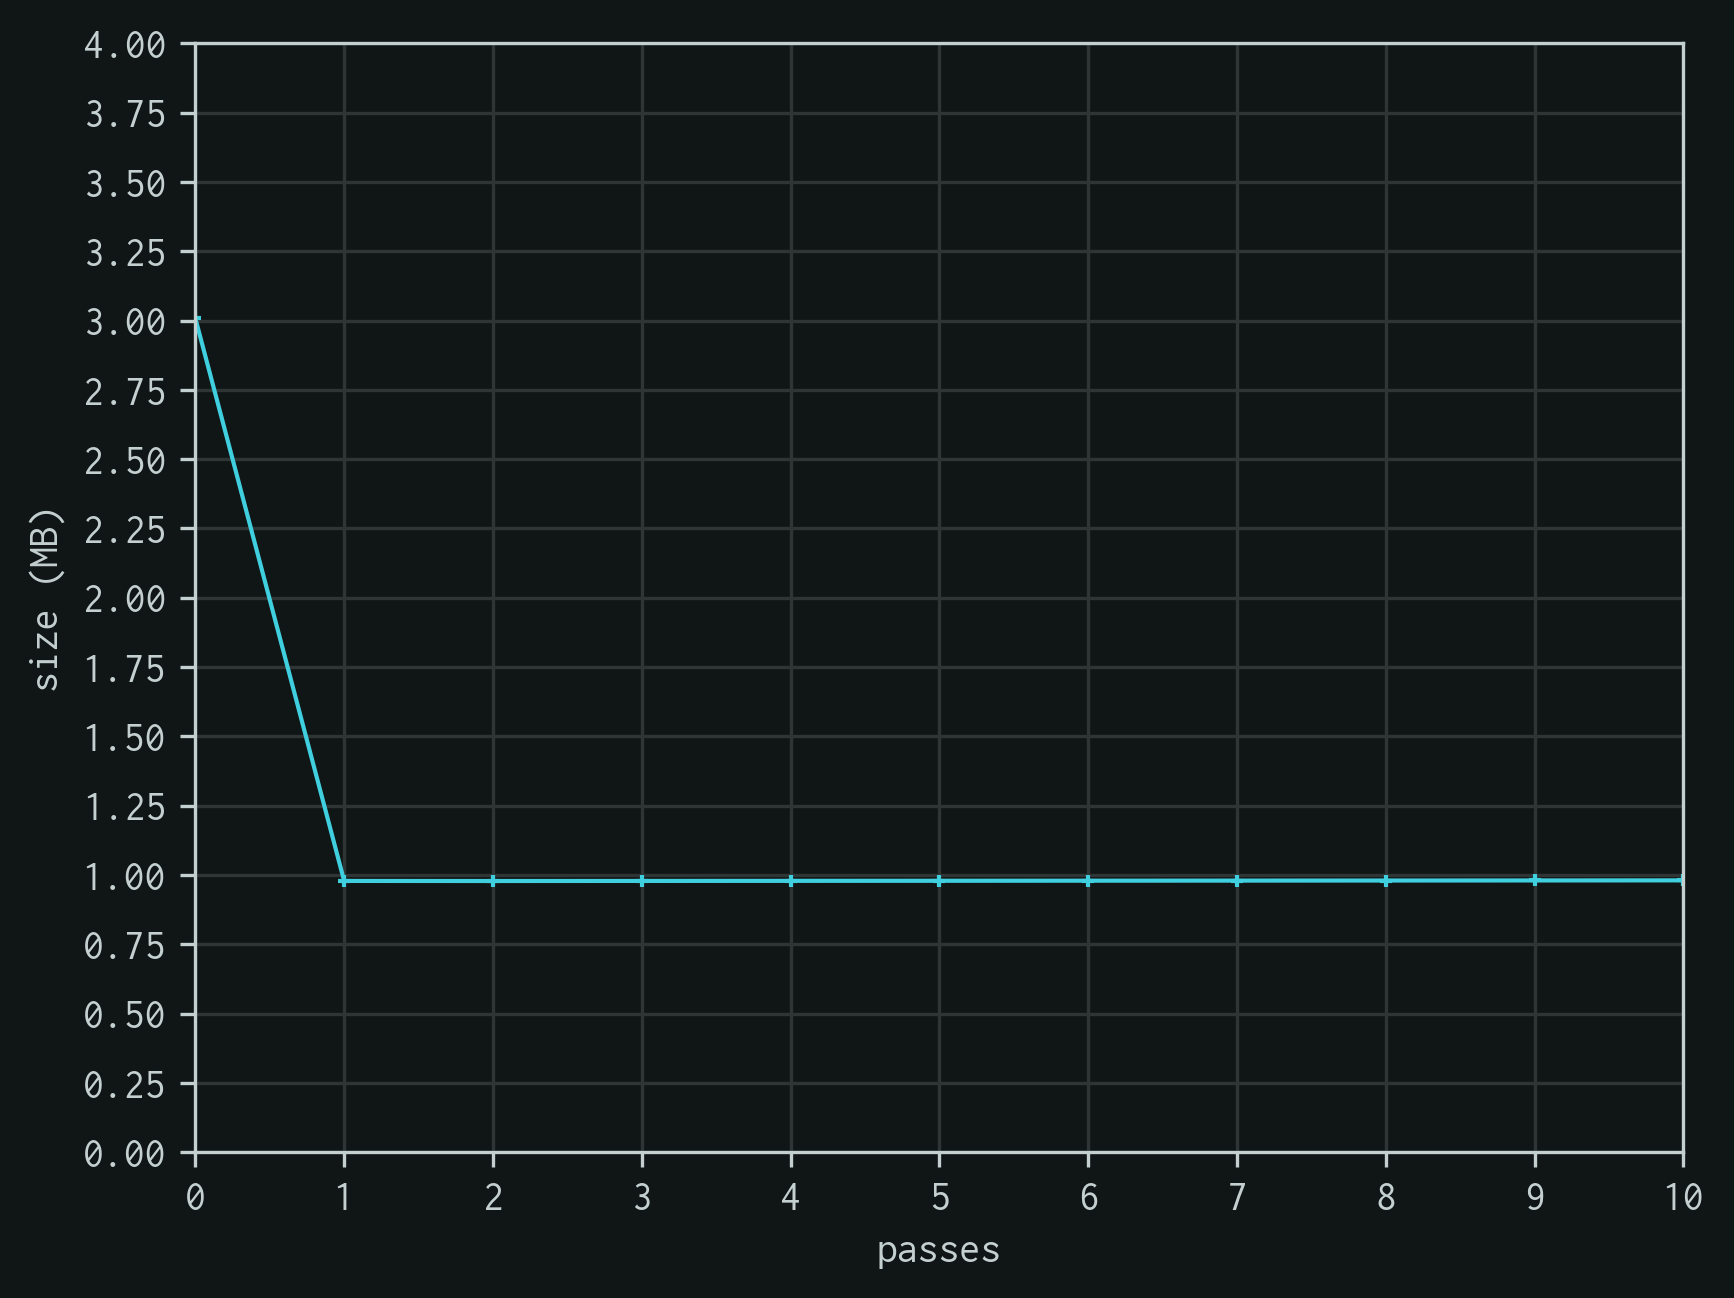
\includegraphics[scale=0.7]{rec_zip.png}
  \end{center}
\end{frame}

\section{Composantes de la compression}

\begin{frame}
  \frametitle{\secname{}}

  \begin{center}
    \tikzset{%
      >={Latex[width=2mm,length=2mm]},
      % Specifications for style of nodes:
      base/.style = {%
        rectangle, rounded corners, draw=minigray, minimum width=6cm,
        minimum height=1.5cm, text centered, font=\sffamily\large},
      transform/.style = {%
        base},
    }
    \begin{tikzpicture}[node distance=2cm,
      every node/.style={fill=extragray, font=\sffamily}, align=center]
      \node (transform) [transform] {(~Transformée~)};
      \pause
      \draw[->] (transform) -- (model);
      \node (model) [base, below of=transform] {\blue{Modèle}};
      \pause
      \draw[->] (model) -- (coding);
      \node (coding) [base, below of=model] {\green{Codage}};
    \end{tikzpicture}
  \end{center}

\end{frame}

\section{Codage}
\subsection{Problème résolu}

\begin{frame}
  \frametitle{\secname{}}
  \framesubtitle{\subsecname{}}
  Le codage, contrairement aux apparences, est un problème \relief{résolu}
  \begin{itemize}
    \item\pause Si les $p_i$ sont connus, la limite de compression théorique est donnée par \sc{Shannon}
    \item\pause \sc{Huffman} permet d'\relief{approcher} cette limite
    \item\pause Le codage arithmétique l'\relief{atteint}
  \end{itemize}
\end{frame}

\begin{frame}
  \frametitle{\secname{}}
  \framesubtitle{\subsecname{}}
  Le codage arithmétique sera détaillé plus loin.

  \relief{Codage d'\sc{Huffman}} pour \tt{turlututu}
  \begin{center}
    \tikzset{%
      >={Latex[width=2mm,length=2mm]},
      % Specifications for style of nodes:
      base/.style = {%
        circle, draw=minigray, text centered,
        font=\sffamily},
    }
    \begin{tikzpicture}[scale=0.9, every node/.style={scale=0.9}]
      \node[draw] at (8, 0) (l_1) [base] {\feuille{1}{l}};
      \node[draw] at (10, 0) (r_1) [base] {\feuille{1}{r}};

      \node[draw] at (13, 1) (t_3) [base] {\feuille{3}{t}};
      \node[draw] at (3, 2) (u_4) [base] {\feuille{4}{u}};
      \pause

      \node[draw] at (9, 1) (empty_2) [base] {\noeud{2}};
      \draw (l_1) -- node[above left, midway] {\bit{0}} (empty_2);
      \draw (r_1) -- node[above right, midway] {\bit{1}} (empty_2);
      \pause

      \node[draw] at (11, 2) (empty_5) [base] {\noeud{5}};
      \draw (empty_2) -- node[above left, midway] {\bit{0}} (empty_5);
      \draw (t_3) -- node[above right, midway] {\bit{1}} (empty_5);
      \pause

      \node[draw] at (7, 3) (empty_9) [base] {\noeud{9}};
      \draw (u_4) -- node[above left, midway] {\bit{0}} (empty_9);
      \draw (empty_5) -- node[above right, midway] {\bit{1}} (empty_9);
      \pause

      \node at (2, 0.75) [above right] {\small\relief{Codes}};
      \node at (2, 0.30) [above right] {\small \bf{\tt{l}}};
      \node at (5, 0.30) [above left] {\bit{100}};
      \node at (2, -0.05) [above right] {\small \bf{\tt{r}}};
      \node at (5, -0.05) [above left] {\bit{101}};
      \node at (2, -0.40) [above right] {\small \bf{\tt{t}}};
      \node at (5, -0.40) [above left] {\bit{11}};
      \node at (2, -0.75) [above right] {\small \bf{\tt{u}}};
      \node at (5, -0.75) [above left] {\bit{0}};
    \end{tikzpicture}
  \end{center}
\end{frame}

\subsection{Inefficacité de \sc{Huffman} -- pourquoi}

\begin{frame}
  \frametitle{\secname{}}
  \framesubtitle{\subsecname{}}
  En pratique, efficacité de \relief{32 \%}
  \pause

  \bigskip

  En appliquant directement \sc{Shannon} aux \relief{fréquences} d'apparition,
  on commet des erreurs
  \begin{itemize}
    \item\pause un symbole n'est pas \relief{indépendant} des précédents
    \item\pause par exemple, en Français, q$\to$\blue{u} est plus fréquent que q$\to$\blue{z}
    \item\pause en quelque sorte, on oublie le caractère \relief{lipschitzien} de nos données
  \end{itemize}
  \pause

  \relief{Il faut donc un modèle}

\end{frame}

\section{Modèles généraux}
\subsection{\tech{bitwise encoder} et \tech{ppm}}

\begin{frame}
  \frametitle{\secname{}}
  \framesubtitle{\subsecname{}}
  \relief{Codage arithmétique} \qquad $p(X_n = \bit{0}) = 0{,}65$
  \begin{center}
  \begin{tikzpicture}[scale=0.8]
  \draw (-1, 0) -- (11, 0);
  \draw (0, 0.25) -- (0, -0.25);
  \draw (10, 0.25) -- (10, -0.25);
  \node at (0, 0.25) [above] {\small $0 = a_0$};
  \node at (10, 0.25) [above] {\small $b_0 = 1$};
  \draw (1.5, 0.25) -- (1.5, -0.25);
  \draw (9, 0.25) -- (9, -0.25);
  \node at (1.5, -0.25) [below] {$a_n$};
  \node at (9, 0.25) [above] {$b_n$};
  \draw (6.375, 0.25) -- (6.375, -0.25);
  \node at (6.375, -0.25) [below] {$\blue{a_{n + 1}}$};
  \node at (6.375, 0.25) [above] {$\green{b_{n + 1}}$};
  \node at (1.5, 0.25) [above] {$\green{a_{n + 1}}$};
  \node at (9, -0.25) [below] {$\blue{b_{n + 1}}$};
  \draw[<->] (1.5, 1.2) -- (6.375, 1.2) [color=regulargreen] node [above, midway] {\color{minigray} $(b_n - a_n) \times p(X_n = \bit{0})$};
  \draw[<->] (6.375, -1.2) -- (9, -1.2) [color=regularblue] node [below, midway] {\color{minigray} $(b_n - a_n) \times p(X_n = \tt{\bf{\blue{1}}})$};
  \end{tikzpicture}
  \end{center}

  \begin{itemize}
    \item\pause Sous-intervalles proportionnels aux \green{$p_i$}
    \item\pause En pratique, avec des $p_i$ non fixes, gérer plus de quelques symboles est compliqué
    \item\pause Implémenté avec des entiers pour représenter $[0 ; 1[$
  \end{itemize}
\end{frame}

\begin{frame}
  \frametitle{\secname{}}
  \framesubtitle{\subsecname{}}

  \relief{\tech{ppm}}
  \begin{itemize}
    \item\pause Le contexte est constitué des $N$ symboles précédents
    \item\pause Un jeu de $p_i$ pour chaque contexte différent
    \item\pause Si le contexte n'a jamais été rencontré, on retombe sur un contexte d'ordre $N - 1$ (\it{order fallback}) etc.
    \item\pause Codage arithmétique
  \end{itemize}
  \pause
  \relief{Inconvénients et solutions}
  \begin{itemize}
    \item\pause Encoder \relief{256} symboles avec des \relief{$p_i$ variables} est dur à implémenter sans pertes
    \item\pause On pourrait donc encoder \relief{bit par bit} au lieu de symbole par symbole
  \end{itemize}
\end{frame}

\subsection{\tech{bitwise ppm} et \tech{bitwise ppm flat}}

\begin{frame}
  \frametitle{\secname{}}
  \framesubtitle{\subsecname{}}
  \relief{\tech{bitwise ppm}}
  \begin{itemize}
    \item\pause Utiliser une \relief{\tech{ppm}} (d'ordre max. 3 octets) avec un encodage \relief{bit par bit}
    \item\pause \relief{49 \%} d'efficacité !
    \item\pause Mais l'\it{order fallback} occasionne des pertes évitables\ldots{}
  \end{itemize}

  \pause
  \relief{\tech{bitwise ppm flat}}
  \begin{itemize}
    \item\pause On retire seulement l'\it{order fallback} en utilisant à la place des probabilités neutres ($0.5 : 0.5$)
    \item\pause Performances améliorées : \relief{63 \%} d'efficacité !
    \item\pause Simplement un \it{bitwise encoder} d'ordre fixe (0 - 28 bits)
  \end{itemize}
\end{frame}

\begin{frame}
  \frametitle{\secname{}}
  \framesubtitle{\tech{bitwise ppm}}

  \vspace{-0.43cm}

  \begin{center}
    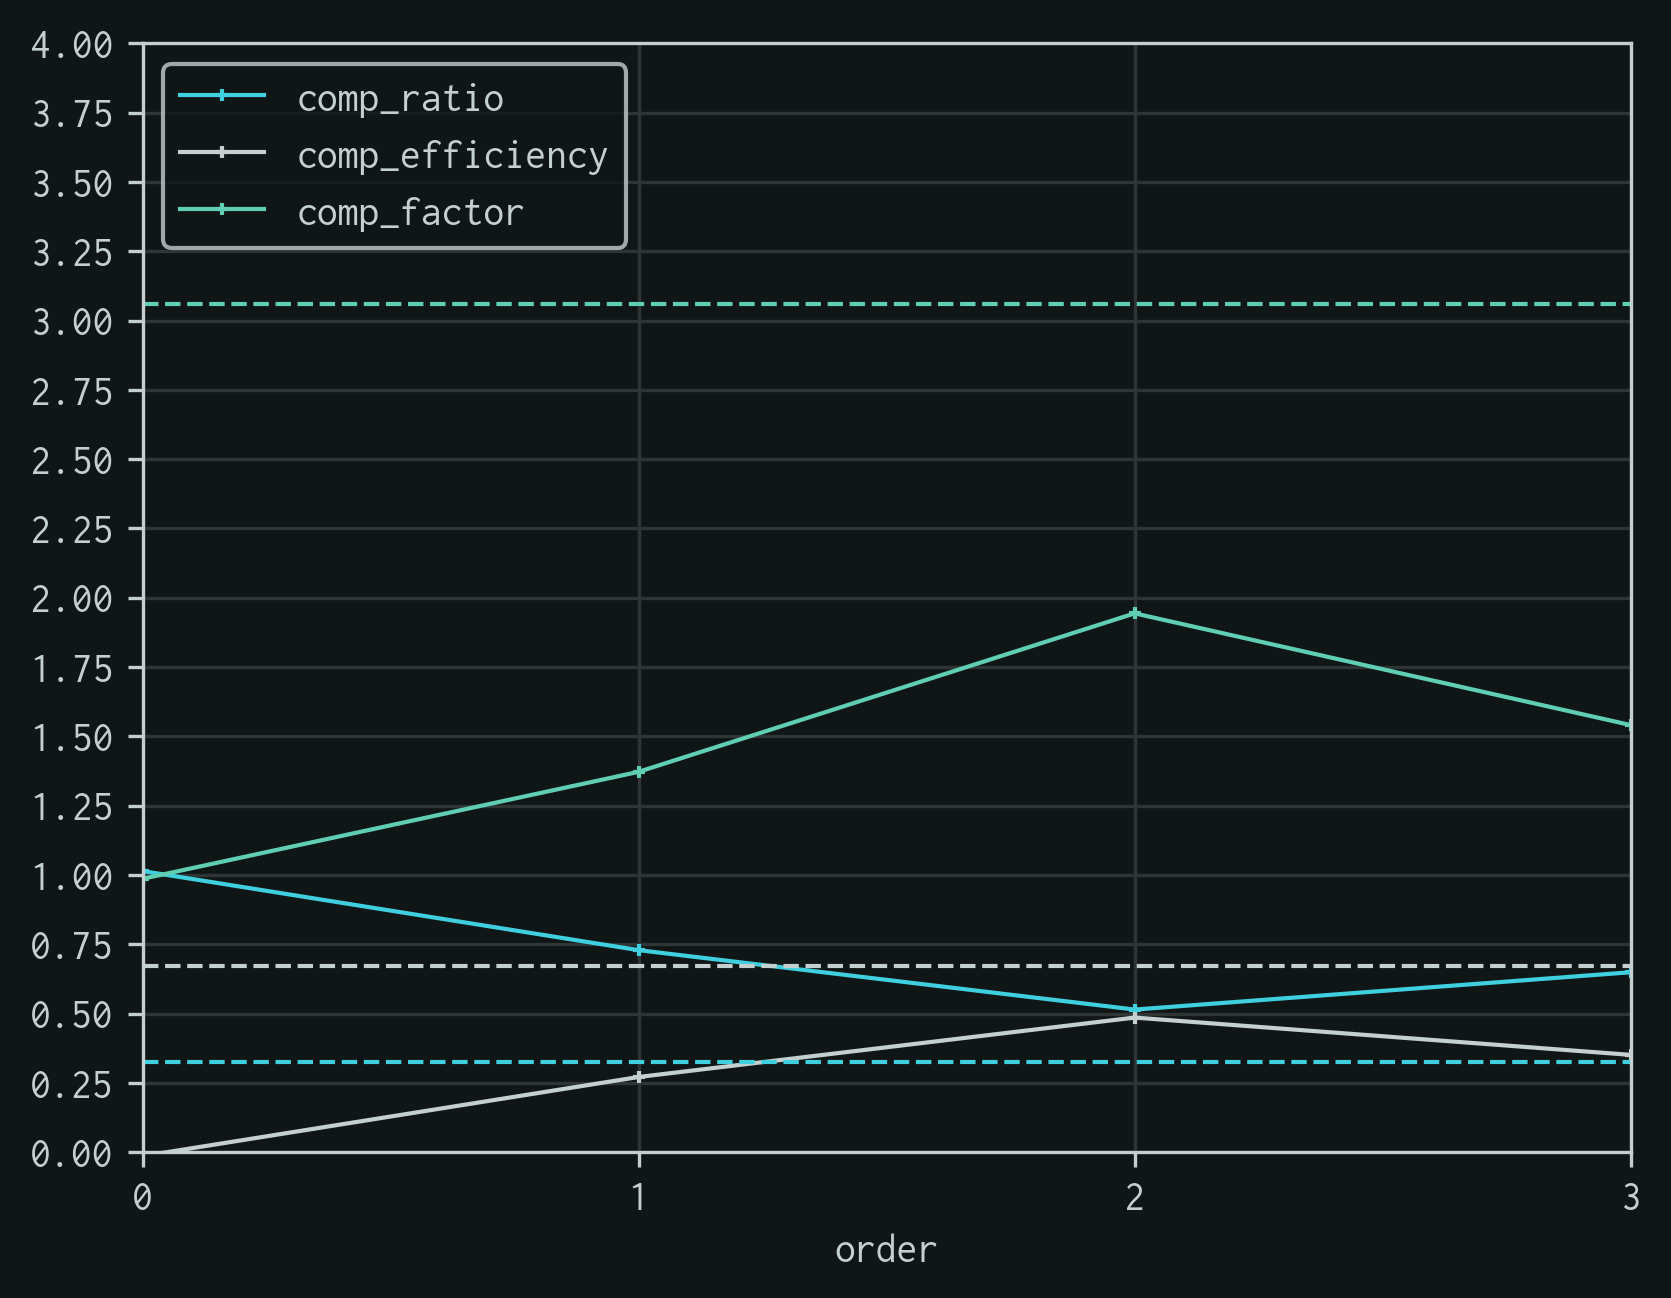
\includegraphics[scale=0.7]{bitwise_ppm.png}
  \end{center}
\end{frame}

\begin{frame}
  \frametitle{\secname{}}
  \framesubtitle{\tech{bitwise ppm flat}}

  \vspace{-0.43cm}

  \begin{center}
    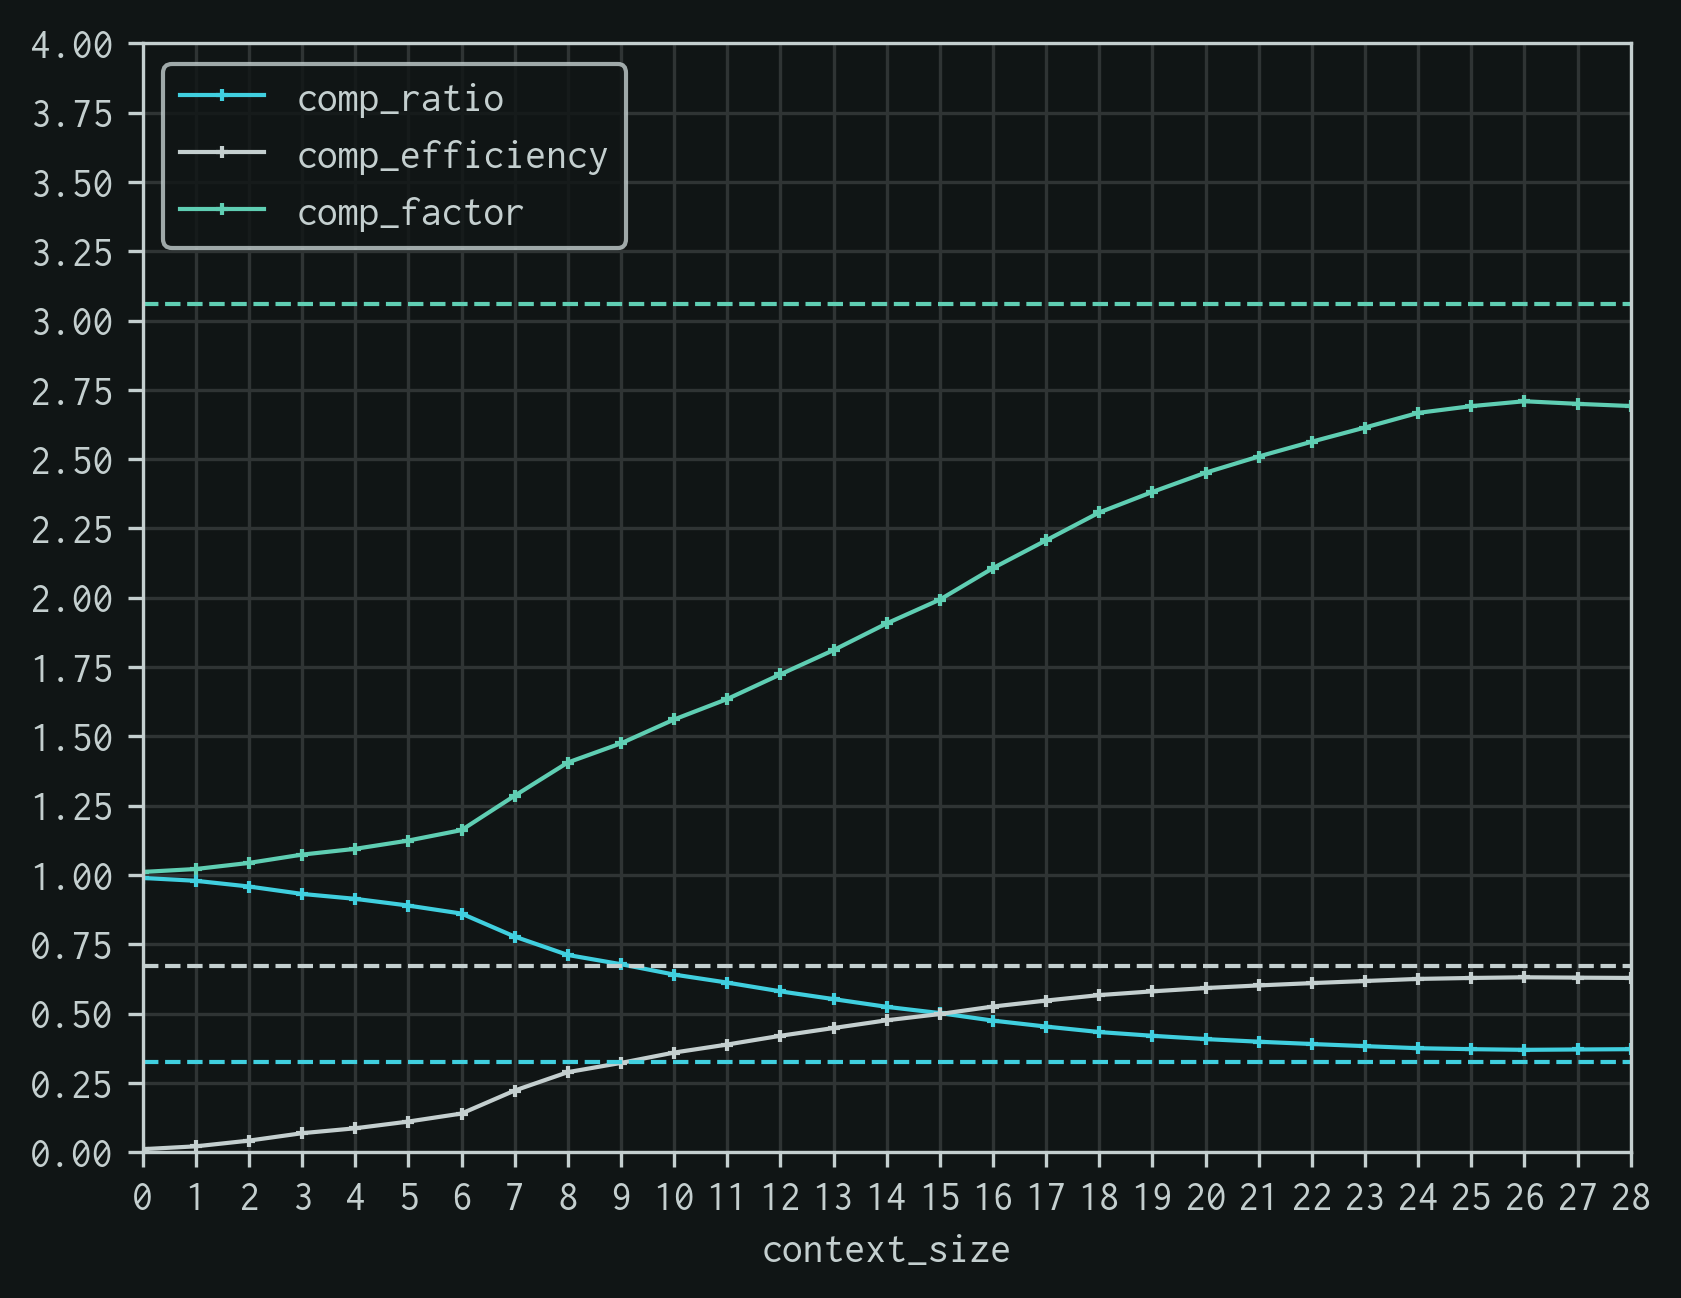
\includegraphics[scale=0.7]{bitwise_ppm_flat.png}
  \end{center}
\end{frame}

\section{Impact de la transformée}
\subsection{\tech{bwt} régularise nos données}

\begin{frame}
  \frametitle{\secname{}}
  \framesubtitle{\subsecname{}}

  \relief{\tech{bwt}}
  \begin{itemize}
    \item\pause Tranformation bijective
    \item\pause Tend à placer côte-à-côte les mêmes symboles
  \end{itemize}

  \pause

\begin{center}

{\ttfamily
\setlength{\tabcolsep}{1.5pt}\renewcommand{\arraystretch}{0.6}
  \begin{tabular}{cccccccccc}
t & u & r & l & u & t & u & t & u & \green{|}\\
\green{|} & t & u & r & l & u & t & u & t & u\\
u & \green{|} & t & u & r & l & u & t & u & t\\
t & u & \green{|} & t & u & r & l & u & t & u\\
u & t & u & \green{|} & t & u & r & l & u & t\\
t & u & t & u & \green{|} & t & u & r & l & u\\
u & t & u & t & u & \green{|} & t & u & r & l\\
l & u & t & u & t & u & \green{|} & t & u & r\\
r & l & u & t & u & t & u & \green{|} & t & u\\
u & r & l & u & t & u & t & u & \green{|} & t\\
  \end{tabular}
\begin{tikzpicture}
  \draw[->] (0, -4) -- (2, -4) node [above, midway] {$\tt{\green{sort}}$};
\end{tikzpicture}
  \begin{tabular}{cccccccccc}
\green{|} & t & u & r & l & u & t & u & t & \blue{u}\\
l & u & t & u & t & u & \green{|} & t & u & \blue{r}\\
r & l & u & t & u & t & u & \green{|} & t & \blue{u}\\
t & u & \green{|} & t & u & r & l & u & t & \blue{u}\\
t & u & r & l & u & t & u & t & u & \green{|}\\
t & u & t & u & \green{|} & t & u & r & l & \blue{u}\\
u & \green{|} & t & u & r & l & u & t & u & \blue{t}\\
u & r & l & u & t & u & t & u & \green{|} & \blue{t}\\
u & t & u & \green{|} & t & u & r & l & u & \blue{t}\\
u & t & u & t & u & \green{|} & t & u & r & \blue{l}\\

  \end{tabular}
}

  \begin{itemize}
    \item\pause $\tech{bwt}(\tt{turlututu}) = \tt{\blue{uruulutttl}}$
    \item\pause Transforme $\green{C^0_m}$ en $\green{C^0}$
  \end{itemize}

\end{center}

\end{frame}

\subsection{La \tech{bwt} en action}

\begin{frame}
  \frametitle{\secname{}}
  \framesubtitle{\subsecname{}}

  \relief{Avec la \tech{rle}}
  \begin{itemize}
    \item\pause Très simple : \blue{\tt{uruulutttl}} devient $1\blue{\tt{u}}\,1\blue{\tt{r}}\,2\blue{\tt{u}}\,1\green{|}\,1\blue{\tt{u}}\,3\blue{\tt{t}}\,1\blue{\tt{l}}$
    \item\pause Efficacité de \relief{41 \%} !
  \end{itemize}

  \pause

  \relief{Avec \tech{bitwise ppm flat}}
  \begin{itemize}
    \item\pause On gagne (seulement) \relief{2 \%} d'efficacité supplémentaire
    \item\pause Permet d'atteindre mon record personnel :\\
    \green{65 \%} d'efficacité \\ facteur de compression \bf{2,85x} \\ \blue{35 \%} de la taille initiale
  \end{itemize}

\end{frame}

\begin{frame}
  \frametitle{\secname{}}
  \framesubtitle{\tech{bwt} + \tech{rle}}

  \vspace{-0.43cm}

  \begin{center}
    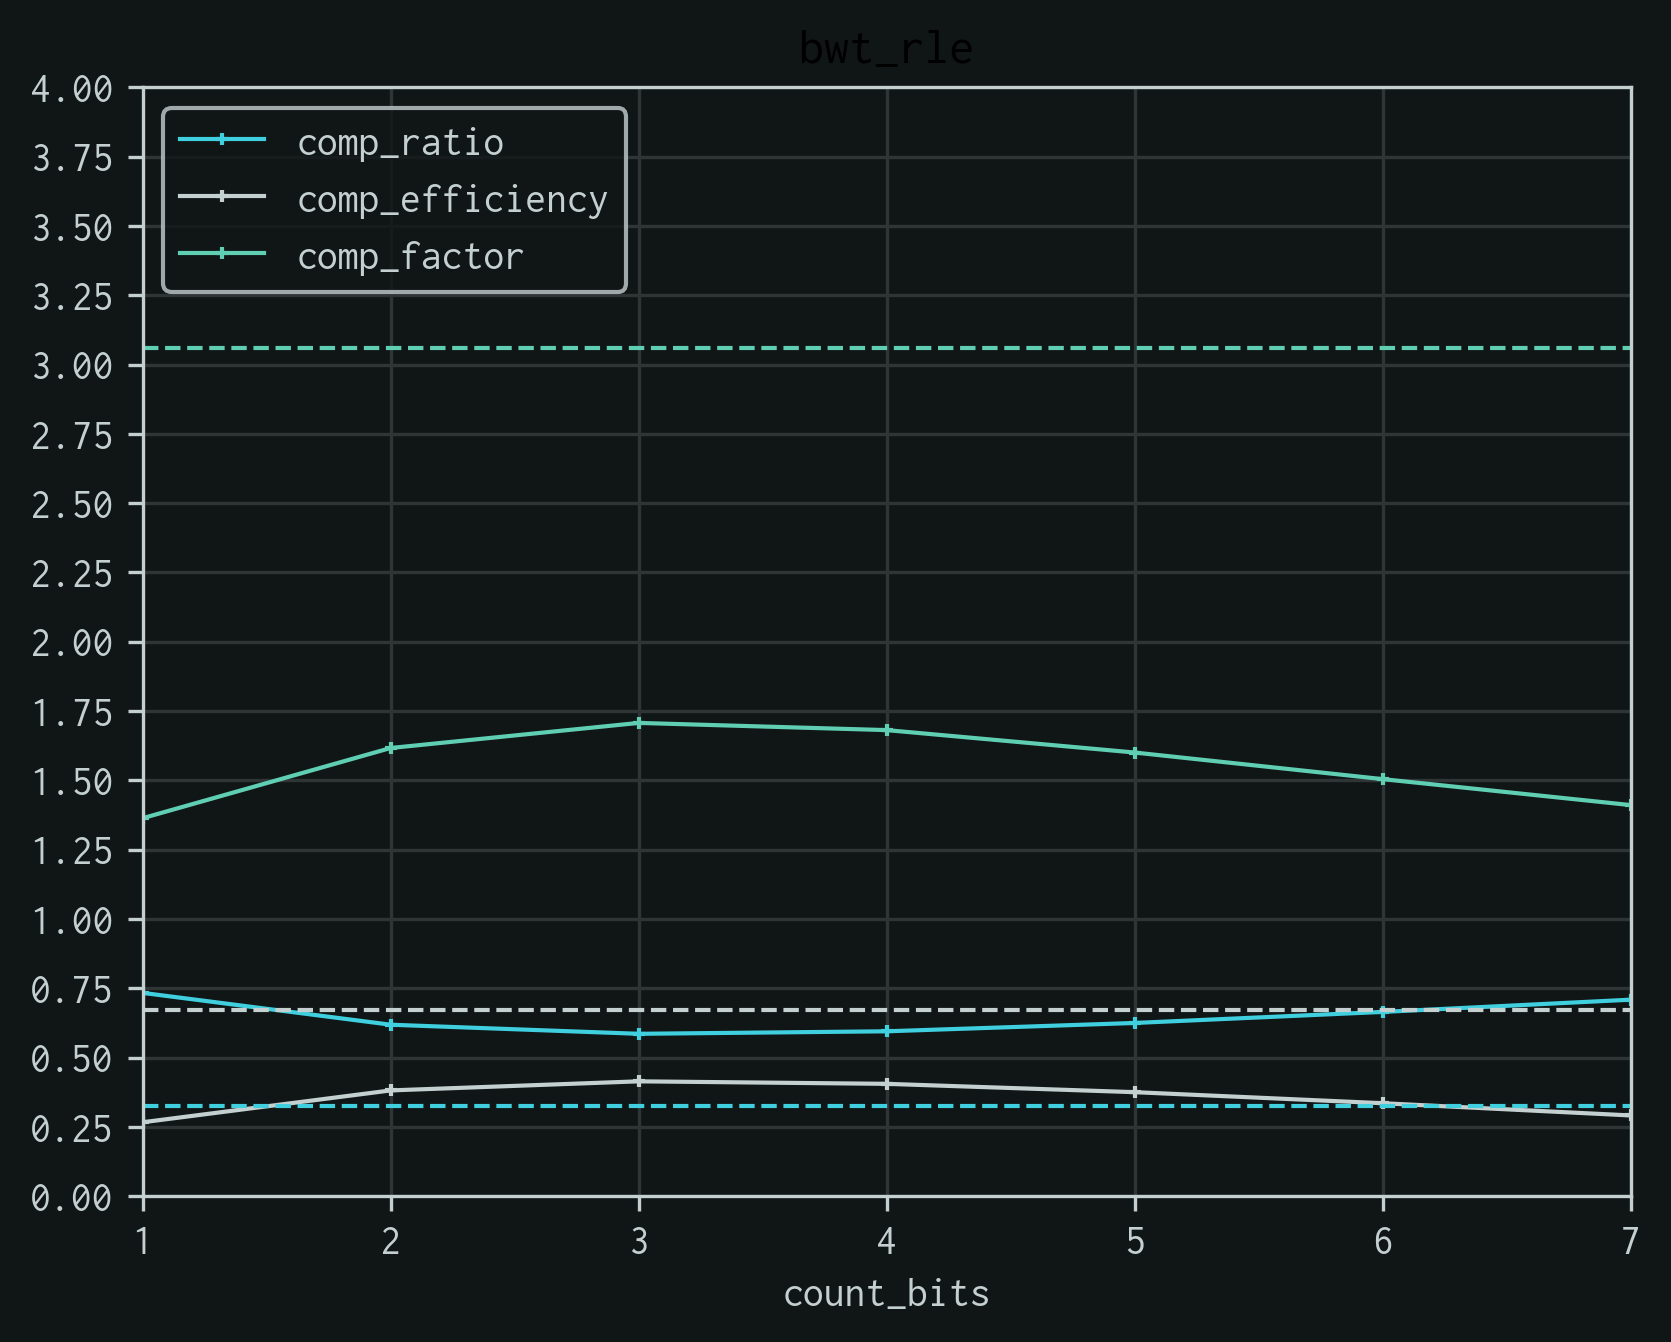
\includegraphics[scale=0.7]{bwt_rle.png}
  \end{center}

\end{frame}

\begin{frame}
  \frametitle{\secname{}}
  \framesubtitle{\tech{bitwise ppm flat} seul (déjà vu)}

  \vspace{-0.43cm}

  \begin{center}
    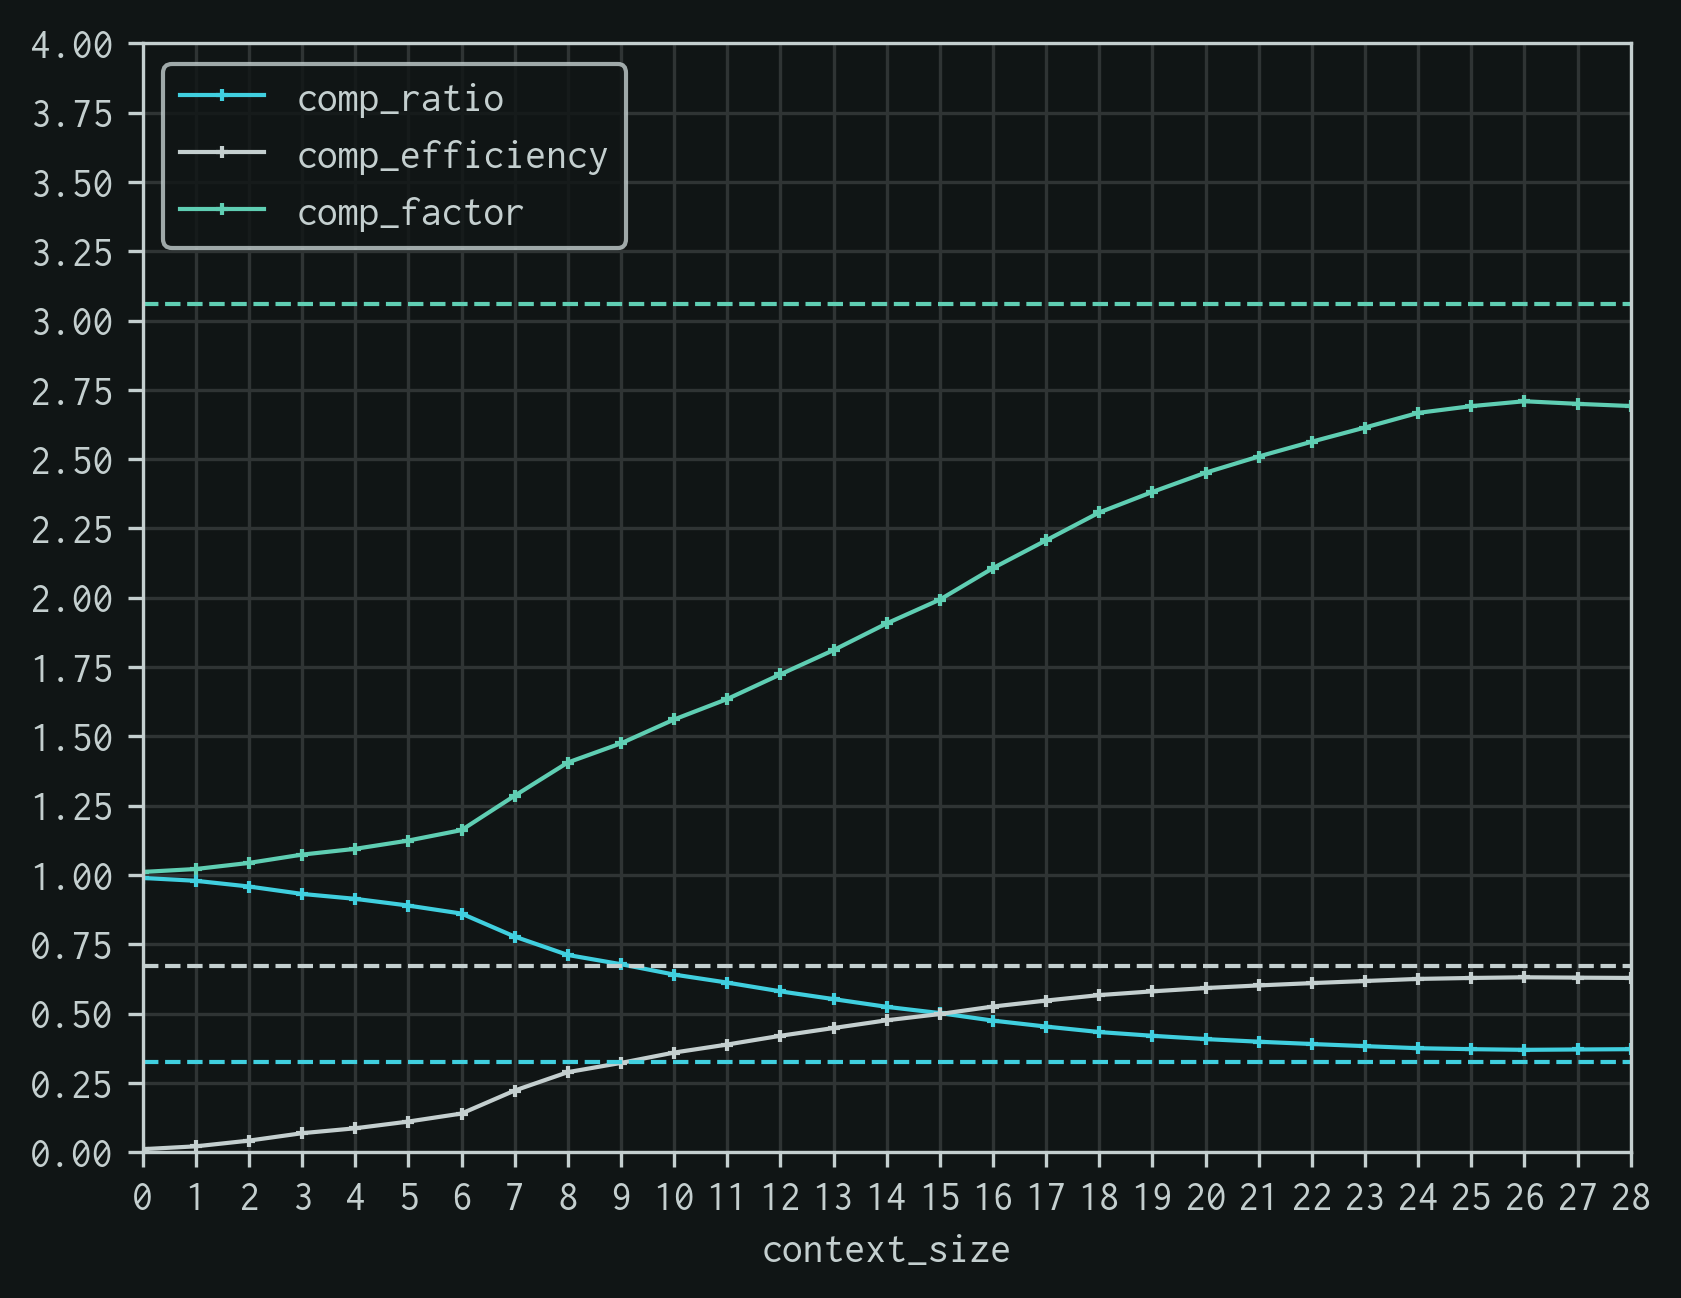
\includegraphics[scale=0.7]{bitwise_ppm_flat.png}
  \end{center}

\end{frame}

\begin{frame}
  \frametitle{\secname{}}
  \framesubtitle{\tech{bwt} + \tech{bitwise ppm flat}}

  \vspace{-0.43cm}

  \begin{center}
    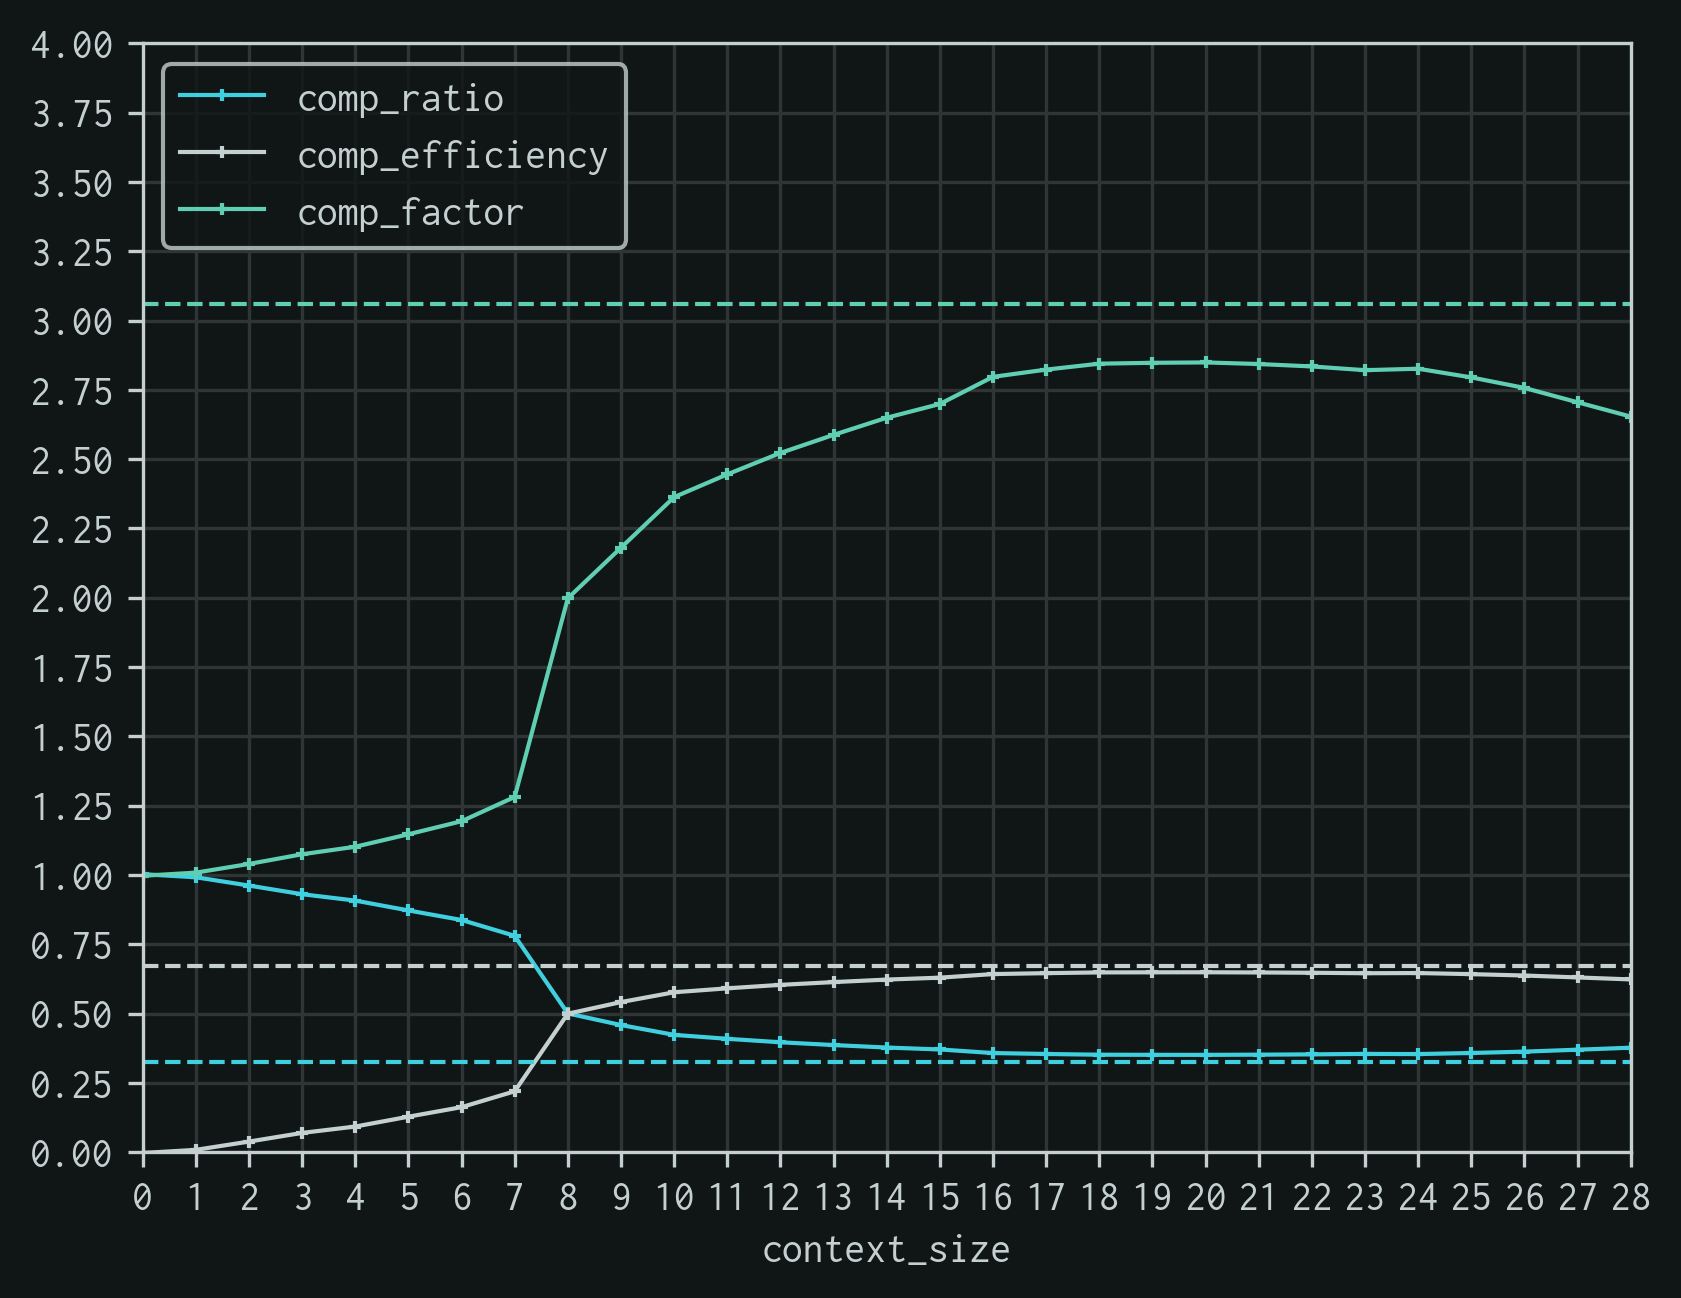
\includegraphics[scale=0.7]{bwt_bitwise_ppm_flat.png}
  \end{center}

\end{frame}

% \section{Résultats finaux}

% \begin{frame}
%   \frametitle{\secname{}}
%   \framesubtitle{\sc{bitwise ppm}}

%   \vspace{-0.43cm}

%   \begin{center}
%     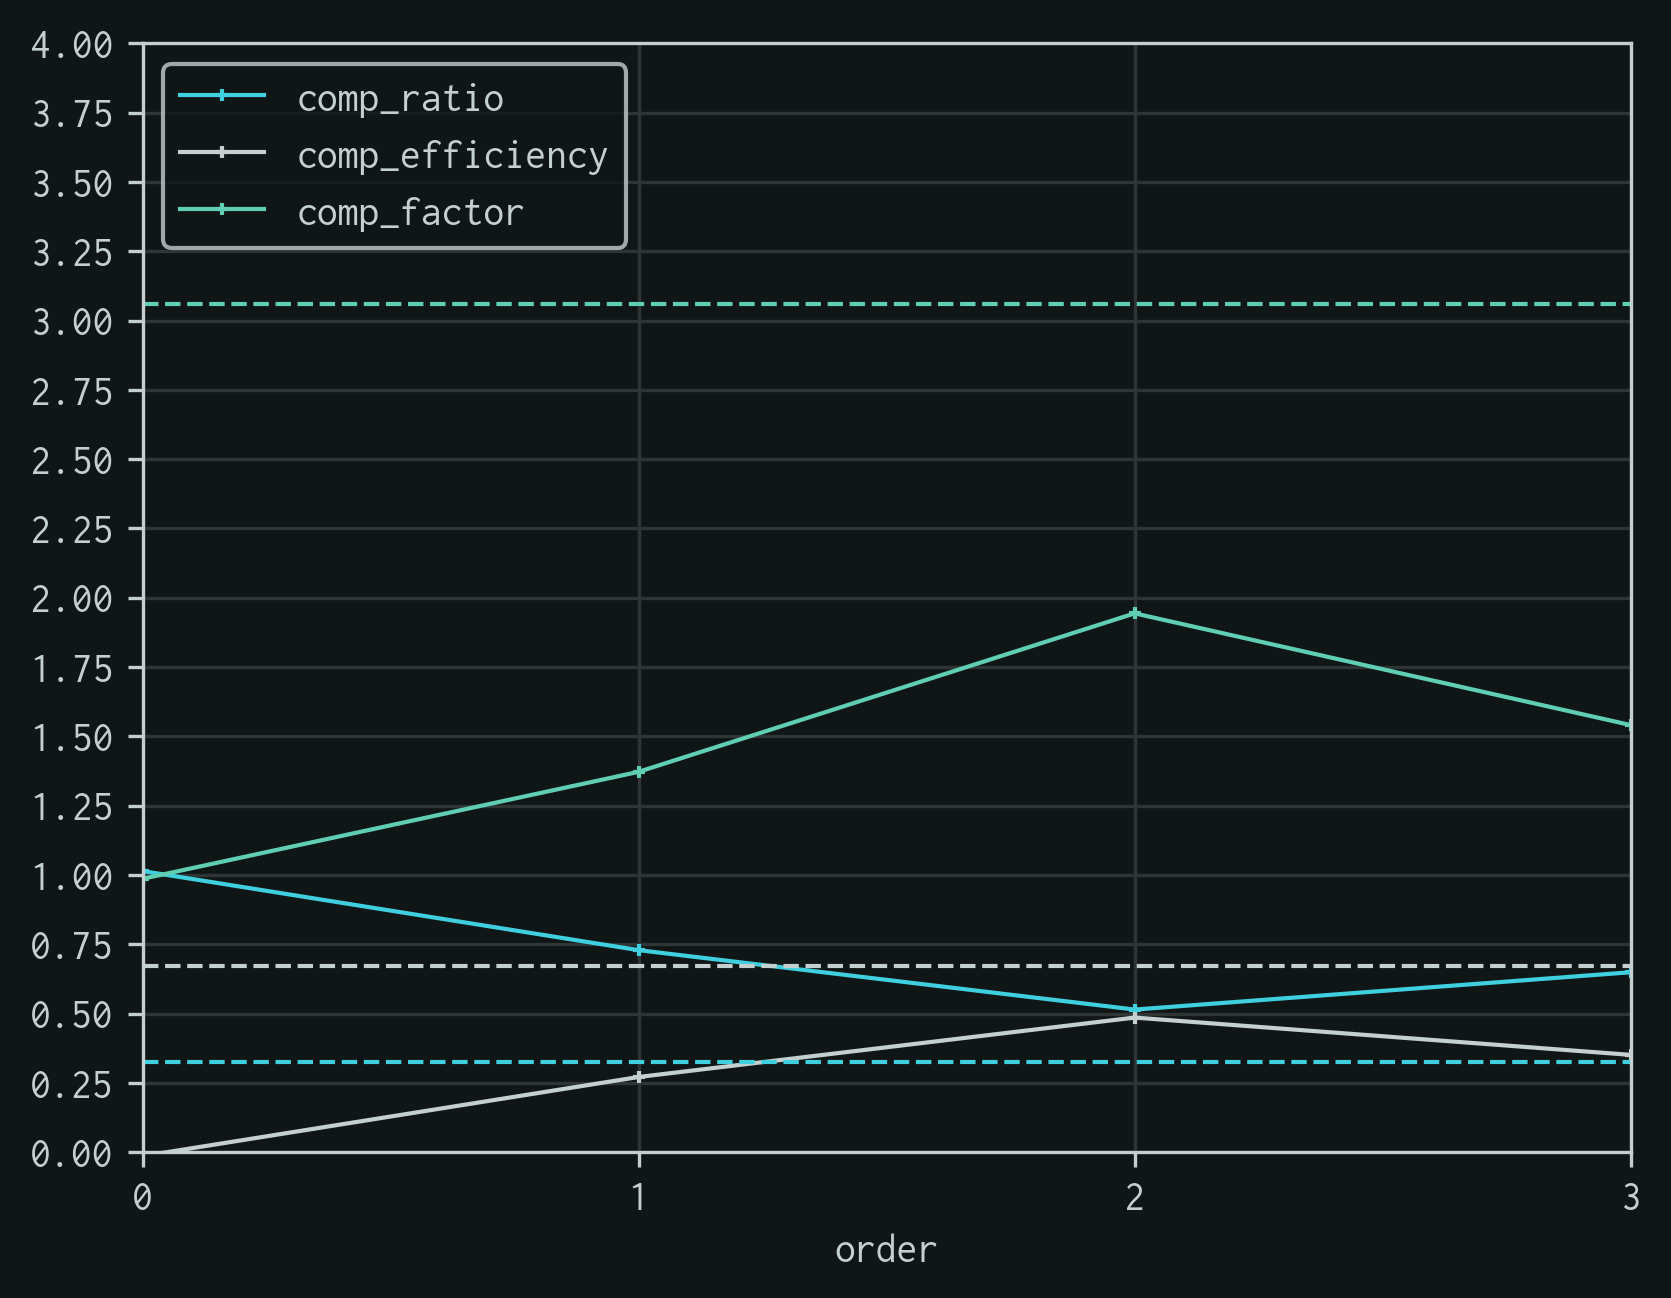
\includegraphics[scale=0.7]{bitwise_ppm.png}
%   \end{center}
% \end{frame}

% \begin{frame}
%   \frametitle{\secname{}}
%   \framesubtitle{\sc{bitwise ppm flat}}

%   \vspace{-0.43cm}

%   \begin{center}
%     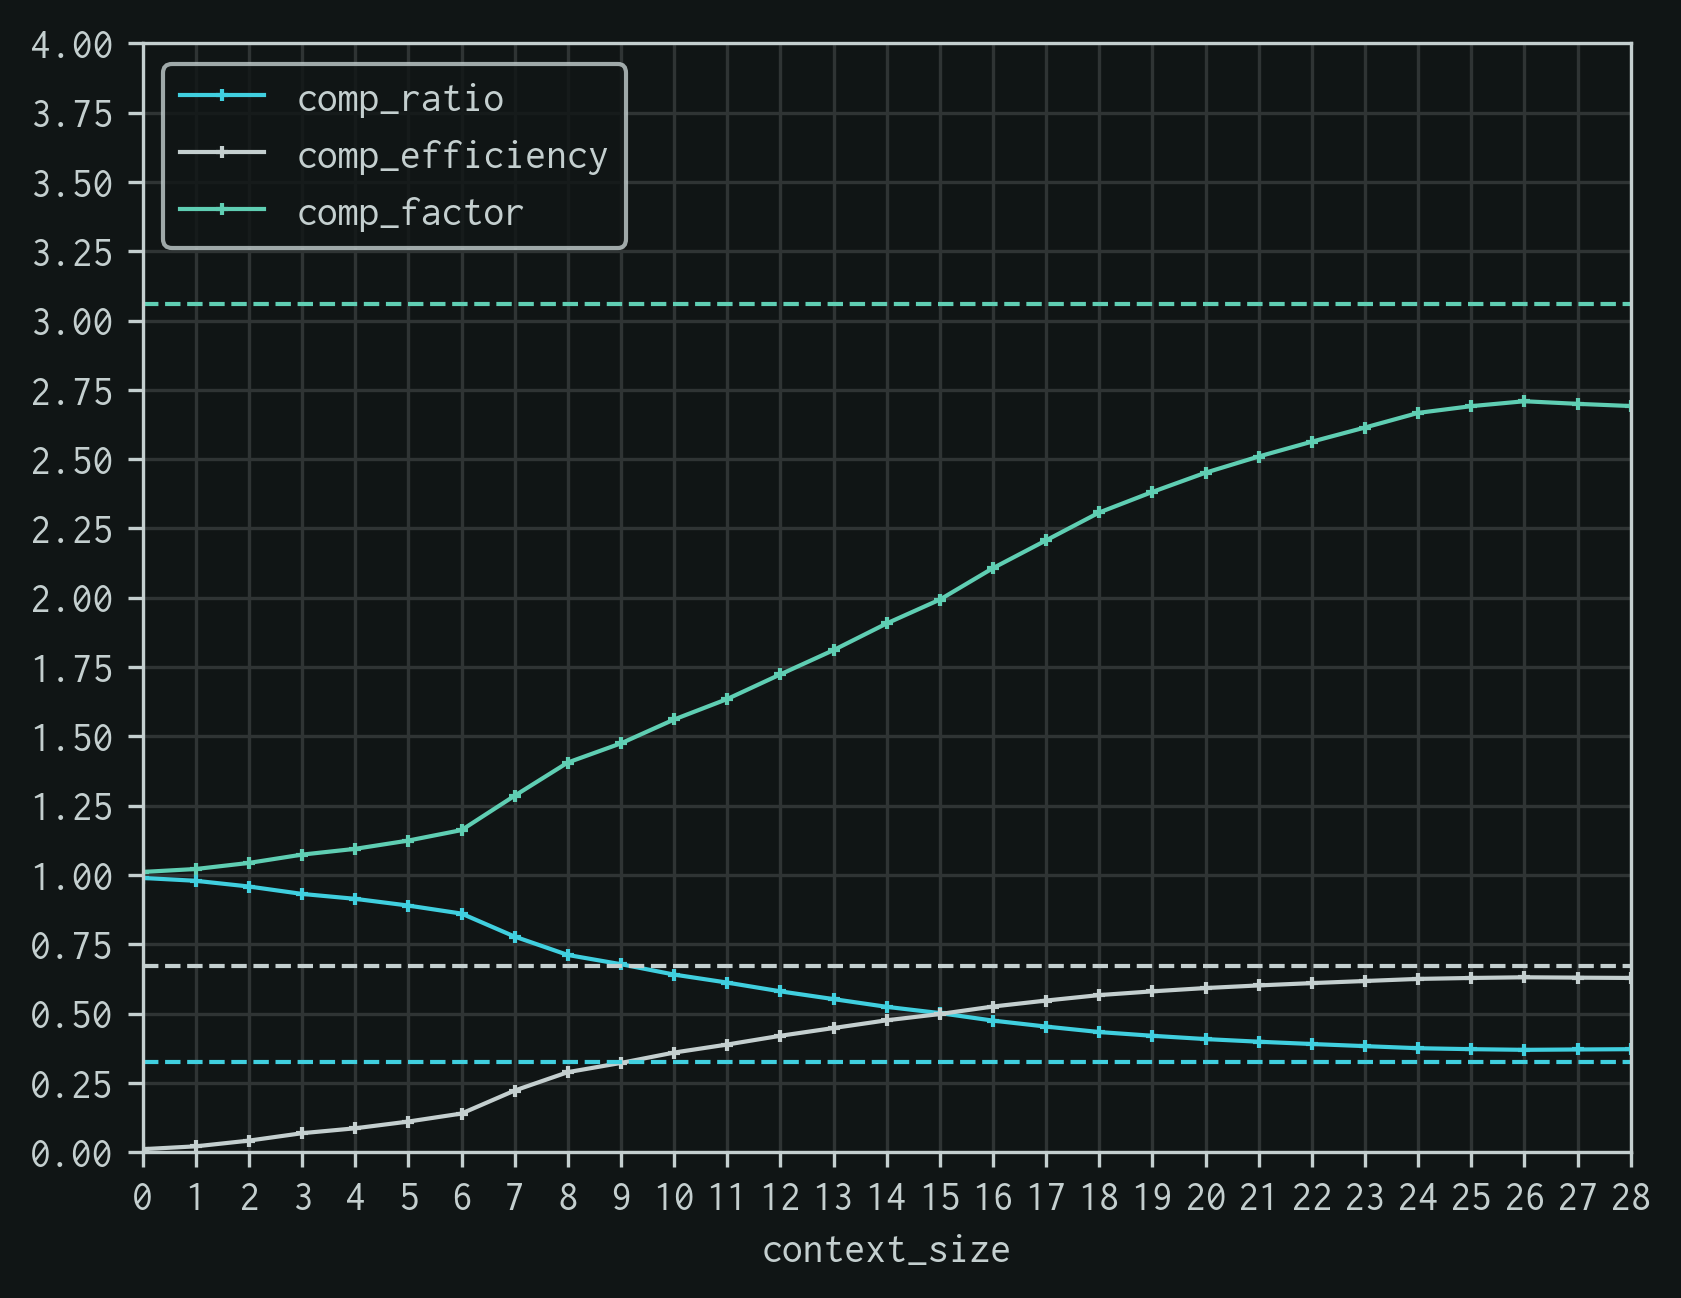
\includegraphics[scale=0.7]{bitwise_ppm_flat.png}
%   \end{center}
% \end{frame}

% \begin{frame}
%   \frametitle{\secname{}}
%   \framesubtitle{\sc{bwt + bitwise ppm flat}}

%   \vspace{-0.43cm}

%   \begin{center}
%     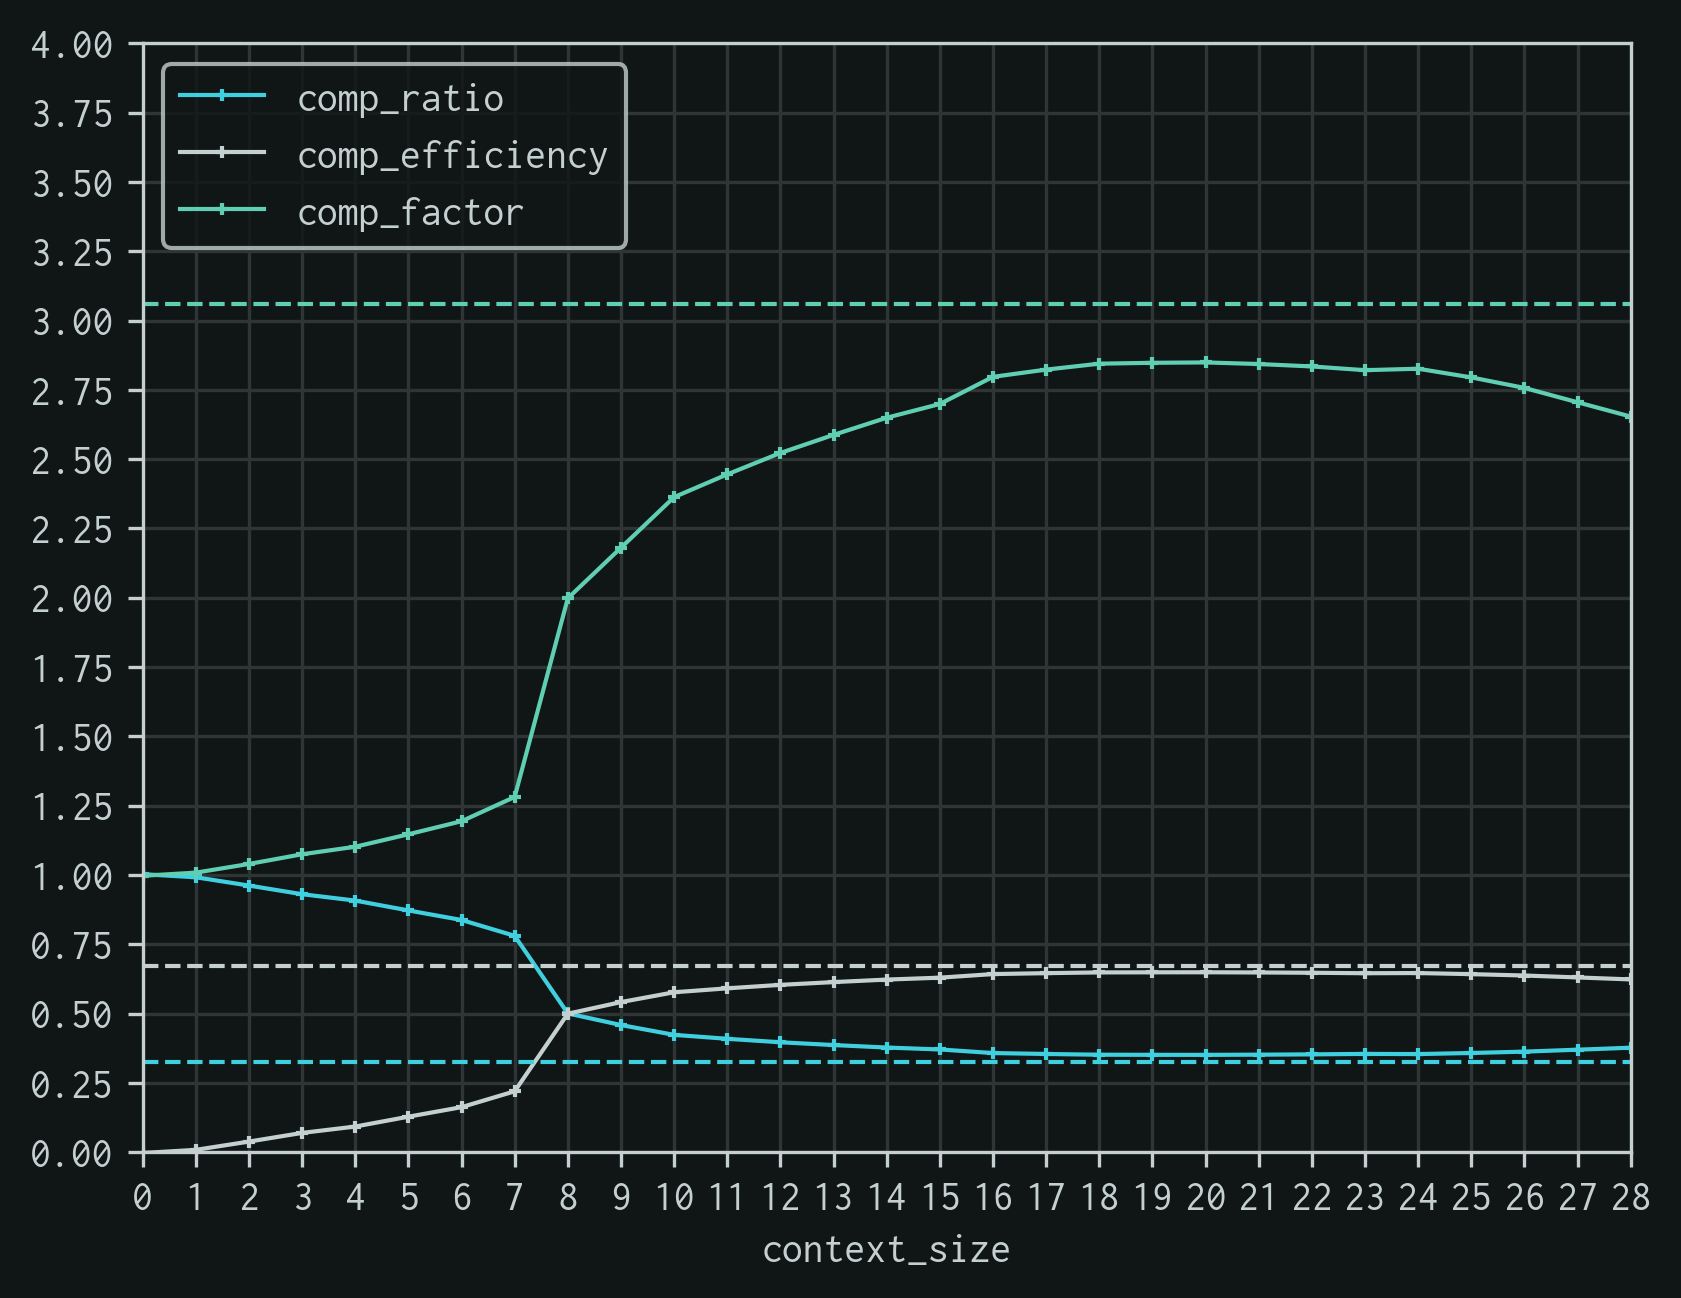
\includegraphics[scale=0.7]{bwt_bitwise_ppm_flat.png}
%   \end{center}
% \end{frame}

% \begin{frame}
%   \frametitle{\secname{}}
%   \framesubtitle{\sc{bwt + rle}}

%   \vspace{-0.43cm}

%   \begin{center}
%     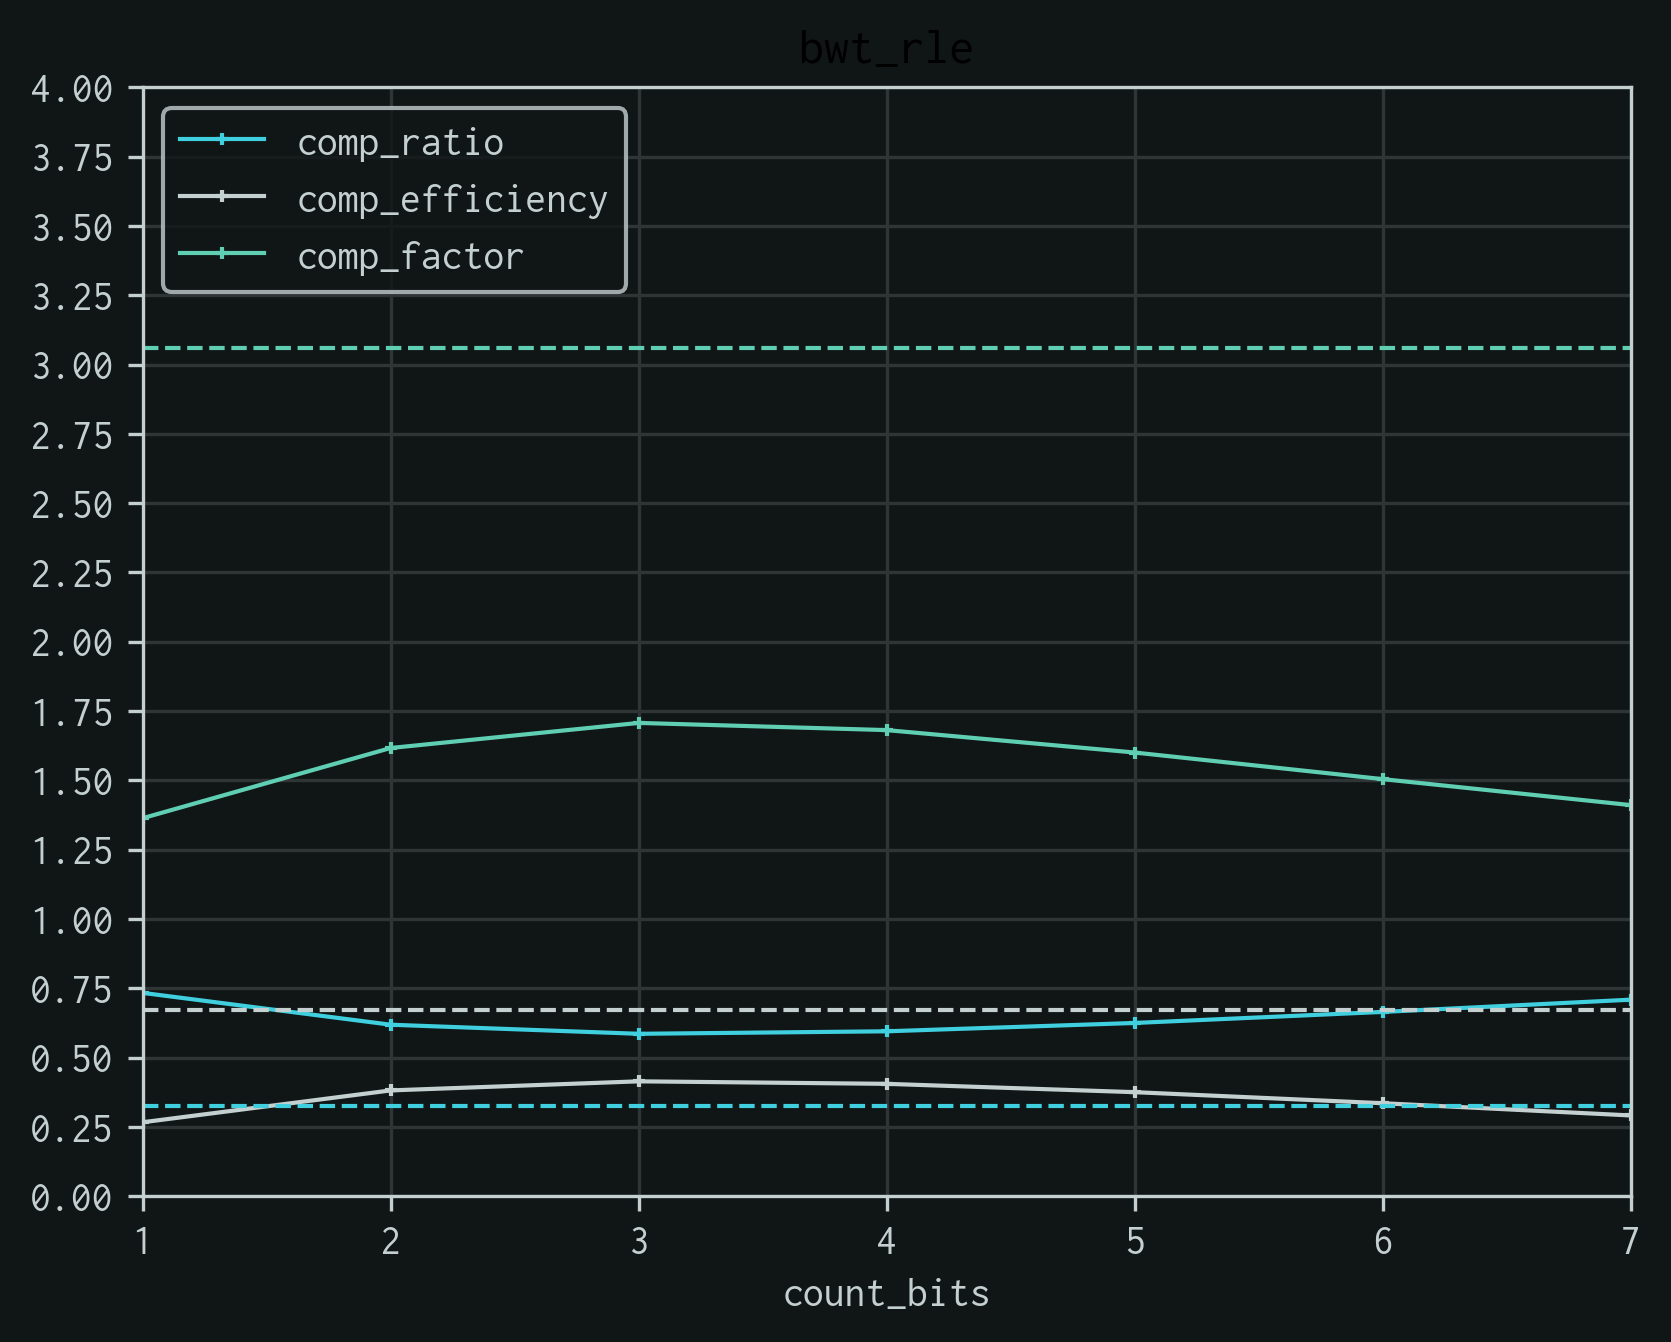
\includegraphics[scale=0.7]{bwt_rle.png}
%   \end{center}
% \end{frame}

\begin{frame}
  \frametitle{Conclusion}
  \framesubtitle{Merci pour votre attention !}

  \relief{Sources principales}
  \begin{itemize}
    \item \it{Data Compression Explained}, Matt \sc{Mahoney} \\
    \url{mattmahoney.net/dc/dce.html}
    \item \it{Suffix Array by Induced Sorting} (pour la \tech{bwt}),\\ G. \sc{Nong}S. \sc{Zhang}, W. H. \sc{Chan}\\
    \url{code.google.com/archive/p/ge-nong/}
  \end{itemize}

  \relief{Tout le dossier disponible}
  \begin{itemize}
     \item {\large \url{https://github.com/tbagrel1/tipe}}
   \end{itemize}

  \begin{center}
    \blue{\rule{0.8\linewidth}{2pt}} \\
    {\small Thomas \sc{Bagrel} - Lycée Henri \sc{Poincaré}, Nancy}
  \end{center}

\end{frame}

\end{document}